%                                                                 aa.dem
% AA vers. 9.1, LaTeX class for Astronomy & Astrophysics
% demonstration file
%                                                       (c) EDP Sciences
%-----------------------------------------------------------------------
%
%\documentclass[referee]{aa} % for a referee version
%\documentclass[onecolumn]{aa} % for a paper on 1 column  
%\documentclass[longauth]{aa} % for the long lists of affiliations 
%\documentclass[letter]{aa} % for the letters 
%\documentclass[bibyear]{aa} % if the references are not structured 
%                              according to the author-year natbib style

%
\documentclass{aa}  

%
\usepackage{showyourwork}

\usepackage{graphicx}
%%%%%%%%%%%%%%%%%%%%%%%%%%%%%%%%%%%%%%%%
\usepackage{txfonts}
\usepackage[utf8]{inputenc} % allow utf-8 input
\usepackage[T1]{fontenc}    % use 8-bit T1 fonts
\usepackage{siunitx}
\usepackage{hyperref}
\usepackage{url}
\usepackage{amsfonts}       % blackboard math symbols
\usepackage{nicefrac}       % compact symbols for 1/2, etc.
\usepackage{microtype}      % microtypography
\usepackage{amsmath}
\usepackage{amssymb}
\usepackage{booktabs}       % professional-quality tables
\usepackage{tabularx}
%%%%%%%%%%%%%%%%%%%%%%%%%%%%%%%%%%%%%%%%
%\usepackage[options]{hyperref}
% To add links in your PDF file, use the package "hyperref"
% with options according to your LaTeX or PDFLaTeX drivers.
%

\usepackage{tikz}

\usepackage{xcolor}

\newcommand{\todo}[1]{\textcolor{red}{#1}}
\newcommand{\T}[1]{\textcolor{orange}{#1}}
%\newcommand{\U}[1]{\textbf{\textit{\textcolor{blue}{#1}}}}
\newcommand{\U}[1]{\textcolor{black}{#1}}
\usepackage{subfigure}

\begin{document} 


   \title{Inferring Galactic Parameters from Chemical Abundances with Simulation-Based Inference}
   
   \titlerunning{Simulation-Based Inference for Galactic Parameters}
   \authorrunning{T. Buck and B. Günes}

   %\subtitle{Inferring Galactic Parameters from Chemical Abundances with Simulation-Based Inference}

   \author{Tobias Buck\inst{1,2}
          \and
          Berkay Günes\inst{1,2}
          }

   \institute{Interdisciplinary Center for Scientific Computing (IWR), University of Heidelberg,
 Im Neuenheimer Feld 205, D-69120 Heidelberg
 \and
 Universität Heidelberg, Zentrum für Astronomie, Institut für Theoretische Astrophysik, Albert-Ueberle-Straße 2, D-69120 Heidelberg, Germany\\
 \email{tobias.buck@iwr.uni-heidelberg.de}
             }

   \date{Received Month, XXXX; accepted Month Day, XXXX}

% \abstract{}{}{}{}{} 
% 5 {} token are mandatory
 \abstract
  % context heading (optional)
  % {} leave it empty if necessary  
   {Chemical abundances of stars are able to reveal important galactic parameters, such as the initial mass function high-mass slope and the frequency of type Ia supernovae. Constraining these parameters is of critical importance in order to create realistic hydrodynamical simulations and understand galactic physics. However, so far inference was significantly limited by the computational cost of traditional Bayesian algorithms. Here we present a new method using simulation-based inference (SBI) to circumvent previous limitations and enable inference from massive stellar surveys.
    SBI enables a new approach to the inference of the posterior distribution of Galactic parameters under an intractable likelihood function by utilizing forward simulations of stellar abundance distributions.
    Using SBI we are able to predict global galactic parameters of great accuracy and precision from chemical abundances of multiple stars, faster than conventional methods like Hamiltonian Monte Carlo inference. Our method easily scales to hundred-thousands of stars and beats previous approaches by orders of magnitude in compute time and accuracy.}
  % aims heading (mandatory)
   {}
  % methods heading (mandatory)
   {}
  % results heading (mandatory)
   {}
  % conclusions heading (optional), leave it empty if necessary 
   {}

   \keywords{Galaxies: fundamental parameters --
            Galaxies: stellar content --
             Methods: data analysis --
             Methods: statistical --
             }
\maketitle
%-------------------------------------------------------------------
\section{Introduction}

Currently all cosmological simulations of galaxy formation \citep[e.g.][]{Sawala2016,Hopkins2018,Pillepich2018,Buck2020,Buck2020c,Font2020,Agertz2021} rely on a small set of galactic parameters to describe fundamental effects of stellar evolution, including the birth and death rates for various types of stars or the production of heavy elements inside stars \citep[e.g.][]{Buck2021}. Two crucial unknowns are the shape of the initial mass function (IMF), setting the mass distribution of stars born from the interstellar medium (ISM), and the rate of Type Ia supernovae (SN\,Ia) explosions.

The exact values of parameters sensitively affect chemical evolution tracks \citep{2005A&A...430..491R,2015MNRAS.449.1327V,2015MNRAS.451.3693M}, yet their observational constraints remain weak.
%
For example, a range of high-mass IMF slopes have been suggested \citep[Tab.\,7]{2016ApJ...824...82C}, with a steeper-than-canonical slope being suggested by a range of studies \citep[e.g.][]{2015ApJ...806..198W,Rybizki2015,Chabrier2014}. In addition, the IMF slope may itself be not a constant but rather a function of metallicity, introducing further complexity \citep[e.g.][]{2019MNRAS.482..118G,Martin2019}. Similarly, the choice of SN\,Ia delay-time-distribution and normalization plays a crucial role in the enrichment of the ISM \citep[e.g.][]{Buck2021} and is heavily debated \citep{2010ApJ...722.1879M,2012MNRAS.426.3282M,2015ApJ...810..137J}. 

The goal of this work is to demonstrate how we can use modern machine learning (ML) techniques in tandem with a simple galactic chemical evolution (GCE) model in a Bayesian framework to infer global galactic parameters from a set of stars. Our work focuses on two key parameters; the high-mass slope of the \citet[Tab.\,1]{2003PASP..115..763C} IMF and the rate of SN\,Ia explosions per unit mass. We assume that both are constant across the galaxy and time.

A methodologically very similar work was previously presented by \cite{Philcox_2019} using Hamilton Monte Carlo sampling for the inference. The result of this work was an impressive speed-up over classical Markov Chain Monte Carlo sampling with no loss of accuracy. Here we make use of simulation-based inference \citep[SBI, e.g.][]{Cranmer2020}. For high-dimensional posterior functions, SBI gives tremendous computational improvements over more traditional methods such as Markov Chain Monte Carlo (MCMC) or even the more efficient Hamilton Monte Carlo (HMC) methods. 

This paper is structured as follows. In Section~\ref{sec:methods} we detail our methods. In particular, we discuss the GCE model and the methods behind SBI. Our results are presented in Section~\ref{sec: Results} where we test the performance of our approach on mock data and data taken from a hydrodynamical simulation. We conclude our study with Section~\ref{sec: conclusion} with a summary and outlook of our results.

\textcolor{red}{to be adapted... especially the zenodo link\\
Finally, we publicly release all of our code to reproduce the results of this manuscript via GitHub\footnote{URL: {\url{https://github.com/TobiBu/sbi-chempy}}}and refer to Appendix \ref{sec:appendix_code_and_data} for an overview of our code and structure. All our datasets and network weights are publicly available on Zenodo.\footnote{URL: \url{https://zenodo.org/record/8375344}}}

\begin{figure*}[]
     \centering
     %\vspace{-.25cm}
     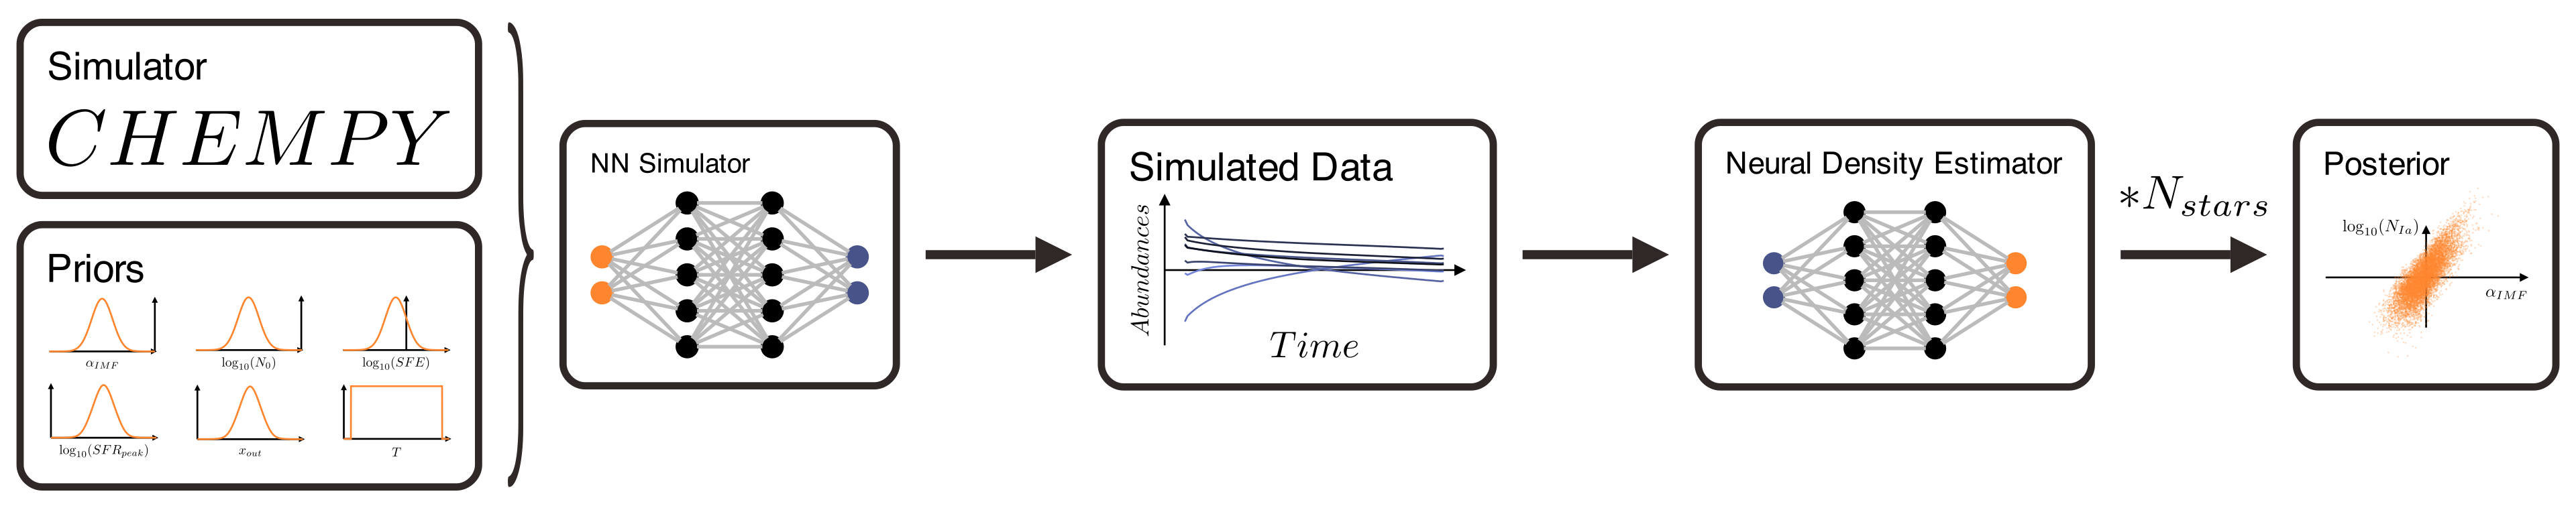
\includegraphics[width=1\linewidth]{figures/sbi_overview.png}
     \vspace{-.5cm}
     \caption{SBI flow chart. From a set of priors we simulate a sample of stellar abundances using \texttt{CHEMPY} \citep{Rybizki_2017,Philcox_2019} which we use to train a \emph{neural network} emulator to speed up the data generation process. Using the \emph{neural network} emulator we produce training data to train the Neural Density Estimator. With this we infer the posterior distribution of the model parameters from a single star. Repeating that for $N_{\rm stars}$ from the same galaxy gives an accurate fit of the IMF slope and Type Ia supernovae normalization.}
     \label{fig:flowchart}
\end{figure*}

% %--------------------------------------------------------------------
\section{Methods}
\label{sec:methods}

In order to establish our new method based on simulation based inference we need two ingredients: A simulator (in our case a Galactic chemical evolution model) that simulates observational data from a set of model parameters (in our case the IMF slope and the Type Ia supernovae normalization) and a flexible way of parametrizing the posterior density conditioned on the observation in order to perform our inference. In the next subsections we describe both ingredients in detail.

\subsection{Galactic chemical evolution models}
Our simulator is based on the \texttt{CHEMPY} model \citep{Rybizki_2017}. \texttt{CHEMPY} is a simple Galactic Chemical Evolution (GCE) model that is able to predict stellar chemical abundances throughout cosmic time by using published nucleosynthetic yield tables for three key processes (SN\,Ia and SN\,II explosions and AGB stellar feedback) and a small number of parameters controlling simple stellar populations (SSPs) and ISM physics. We refer to the initial \texttt{CHEMPY} paper \citep{Rybizki_2017} for the details of the model.

In particular, we are using the \texttt{CHEMPYScoring} module \citep{Philcox_2018} publicly available as the \texttt{CHEMPYMulti} \citep{Philcox_2019}\footnote{\href{https://github.com/oliverphilcox/ChempyMulti}{github.com/oliverphilcox/ChempyMulti}} package a further development of the original \texttt{CHEMPY} model. 

\paragraph{\texttt{CHEMPY} parameters}
In this work, we allow six \texttt{CHEMPY} parameters to vary freely (see also Tab.\,\ref{tab:priors}). These can be categorized into three groups:
\begin{enumerate}
     \item $\vec\Lambda$: \textbf{Global Galactic Parameters} describe SSP physics and comprise the high-mass \citet{2003PASP..115..763C} IMF slope, $\alpha_\mathrm{IMF}$, and (logarithmic) Type Ia SN normalization, $\log_{10}(N_\mathrm{Ia})$. We treat these as star-independent and assume them to be constant across galactic environments and cosmic time\footnote{Whilst $\log_{10}(N_\mathrm{Ia})$ is constant with respect to time by definition, it being simply a normalization constant, there is some evidence for $\alpha_\mathrm{IMF}$ varying as a function of time or metallicity \citep{Chabrier2014,2016MNRAS.462.2832C,2019MNRAS.482..118G,Martin2019}.}. 
     We adopt the same broad priors as \citep{Philcox_2019} for these variables (see also Tab.\ref{tab:priors}). 
     %
     \item $\{\vec\Theta_i\}$: \textbf{Local Galactic Parameters} describe the local physics of the ISM and are hence specific to each stellar environment, indexed by $i$. As defined in \citep{Rybizki_2017}, these include the star-formation efficiency (SFE), $\log_{10}(\text{SFE})$, $\log_{10}(\mathrm{SFR}_\mathrm{peak})$, which controls the peak of the star formation rate (SFR), and the fraction of stellar outflow that is fed to the gas reservoir, $\mathrm{x}_\mathrm{out}$. We adopt broad priors for all parameters and, as in \citep{Philcox_2019}, fix the SN\,Ia delay-time distribution, $\log_{10}(\tau_{\rm Ia})$, to $\log_{10}(\tau_{\rm Ia})=-0.80$ \citep[see also][]{Philcox_2018}.
     \item $\{T_i\}$: \textbf{Stellar Birth-Times}. Time in Gyr at which a given star is formed from the ISM. We assume that its proto-stellar abundances match the local ISM abundances at $T_i$.
\end{enumerate}

The separability of local (ISM) parameters and global (SSP) parameters is motivated by recent observational evidence: \citet{2019arXiv190710606N} find that the elemental abundances of red clump stars belonging to the thin disk can be predicted almost perfectly from their age and [Fe/H] abundance. This implies that the key chemical evolution parameters affecting the elemental abundances (SSP parameters and yield tables) are held fixed, whilst ISM parameters vary smoothly over the thin disk \citep[which offsets the metallicity for different galactocentric radii, e.g.][for a simulated example]{Buck2020, Wang2024}. Similarly \cite{2019ApJ...874..102W} find that ISM parameter variations are deprojected in the [X/Mg] vs [Mg/H] plane (their Fig.\,17) and that abundance tracks in that space are independent of the stellar sample's spatial position within the Galaxy (their Fig.\,3).

Following \citet{Philcox_2019}, to avoid unrealistic star formation histories (that are very `bursty' for early stars), we additionally require that the SFR (parametrized by a $\Gamma$ distribution with shape parameter $a=2$) at the maximum possible stellar birth-time ($13.8$\,Gyr) should be at least 5\% of the mean SFR, ensuring that there is still a reasonable chance of forming a star at this time-step. This corresponds to the constraint $\log_{10}\left(\mathrm{SFR}_\mathrm{peak}\right)>0.294$. For this reason, a truncated Normal prior will be used for the SFR parameter. Furthermore, we constrain $T_i$ to the interval $[1,13.8]$\,Gyr (assuming an age of the Universe of 13.8\,Gyr), ignoring any stars formed before $1$\,Gyr, which is justified as these are expected to be rare.


\begin{tiny}
\begin{table*}
\begin{minipage}{\textwidth}
\begin{center}
\caption{Free \texttt{Chempy} parameters for each star, with their prior values and Gaussian widths. Stellar birth-times are set for each star individually from a Uniform prior, based on realistic age estimates.}
\begin{tabularx}{\textwidth}{ >{\raggedleft}p{2.2cm}p{6.5cm}|c c }
Parameter & Description & $\overline{\theta}_\mathrm{prior}\pm\sigma_\mathrm{prior}$ & Prior from: \\

\hline
\multicolumn{4}{c}{$\vec{\Lambda}$: \textit{Global stellar (SSP) parameters}}\\
\hline
$\alpha_\mathrm{IMF}$ & High-mass slope of the \citep{2003PASP..115..763C} IMF & $-2.3\pm0.3$ & \citep[Tab.\,1]{2003PASP..115..763C} \\
  
$\log_{10}\left(N_\mathrm{Ia}\right)$ & Number of SN\,Ia per $\mathrm{M}_\odot$ over 15\,Gyr & $-2.75\pm0.3$ & \citep[Tab.1\,]{2012PASA...29..447M}\\
  
\hline
\multicolumn{4}{c}{$\vec{\Theta}_i$: \textit{Local ISM parameters}}\\
  
\hline
$\log_{10}\left(\mathrm{SFE}\right)$ & Star formation efficiency governing gas infall & $-0.3\pm0.3$ & \citep{2008AJ....136.2846B}\\
  
$\log_{10}\left(\mathrm{SFR}_\mathrm{peak}\right)$ & SFR peak in Gyr (scale of $k=2$ $\Gamma$-distribution) & $0.55\pm0.1$ & \citep[fig.\,4b]{2013ApJ...771L..35V}\\
  
x$_\mathrm{out}$ & Stellar feedback fraction & $\phantom{-}0.5\pm0.1$ & \citep[Tab.\,1]{Rybizki_2017}\\
  
\hline
\multicolumn{4}{c}{$T_i$: \textit{Timescale}}\\
 
\hline
$T_i$ & Time of stellar birth in Gyr & [$1$,$13.8$] & Observations

\label{tab:priors}
\end{tabularx}
\end{center}
\end{minipage}
\end{table*}
\end{tiny}

\paragraph{Nucleosynthetic yield tables}
We adopt the same nucleosynthetic yield tables as in \citep{Philcox_2019}, see their Sec.~2.2 for more details.
To test our method, we aim further at inferring parameters from a sample of stars taken from a hydrodynamical simulation of a MW type galaxy which we take from the Ilustris TNG project \citep{Pillepich2018}. To ensure maximal compatibility with TNG, we adopt their nucleosynthetic yield tables in \texttt{Chempy}, for enrichment by SN\,Ia, SN\,II and AGB stars. The utilized yields are summarized in Tab.\,\ref{tab:chempy_TNG_yields}, matching \citet[Tab.\,2]{2018MNRAS.473.4077P}, and we note that the SN\,II yields are renormalized such that the IMF-weighted yield ratios at each metallicity are equal to those from the \citet{2006ApJ...653.1145K} mass range models alone. \texttt{Chempy} uses only net yields, such that they provide only newly synthesized material, with the remainder coming from the initial SSP composition. These tables may not well-represent true stellar chemistry, and the effects of this missmatch are examined in Sec.\,\ref{subsec: mocks_wrong_yield} by performing inference using an alternative set of yields that does not match the yield set of the training data. For the analysis of observational data, we would want to use the most up-to-date yields, such as \citet{2016ApJ...825...26K} AGB yields, and carefully chose elements which are known to be well reproduced by our current models (e.g. shown by \citet{2019ApJ...874..102W,2019arXiv190806113G}), though this is not appropriate in our context. To facilitate best comparison with TNG, we further set the maximum SN\,II mass as $100\,\mathrm{M}_\odot$ (matching the IMF upper mass limit), adopt stellar lifetimes from \citet{1998A&A...334..505P} and do not allow for any `hypernovae' \citep[in contrary to][]{2018ApJ...861...40P}).

\begin{table}[]
\caption{Nucleosynthetic yield tables used in this analysis, matching those of the TNG simulation \citep[Tab.\,2]{2018MNRAS.473.4077P}.}
     \centering
     \begin{tabular}{c|c}
       Type & Yield Table \\
        \hline
         SN\,Ia & \citet{1997NuPhA.621..467N}\\
         SN\,II & \citet{2006ApJ...653.1145K,portinari}\\
         AGB & \citet{2010MNRAS.403.1413K,2014MNRAS.437..195D};\\
         & \citet{2014ApJ...797...44F}
     \end{tabular}
 \label{tab:chempy_TNG_yields}
 \end{table}


\paragraph{Chemical elements}
In our analysis we only track nine elements: C, Fe, H, He, Mg, N, Ne, O and Si since these are the only elements traced by TNG. We principally compare the logarithmic abundances [X/Fe] and [Fe/H] defined by 
\begin{equation}
     [\mathrm{X}/\mathrm{Y}] = \log_{10}(N_\mathrm X/N_\mathrm Y)_\mathrm{star} - \log_{10}(N_\mathrm X/N_\mathrm Y)_\odot
\end{equation}
for number fraction $N_\mathrm X$ of element X. Here $\odot$ denotes the solar number fractions of \citet{2009ARA&A..47..481A}. This uses H for normalization, thus we are left with $n_\mathrm{el}=8$ independent elements which must be tracked by \texttt{Chempy}\footnote{In observational contexts, it may be more appropriate to compute abundances relative to Mg rather than Fe (as in \citep{2019ApJ...874..102W}) since Mg is only significantly produced by SN\,II and hence a simpler tracer of chemical enrichment.}. 

With these modifications, \texttt{Chempy} allows for fast prediction of TNG-like chemical abundances for a given set of galactic parameters. It is important to note that the two GCE models have very different parametrizations of galactic physics, with TNG including vastly more effects, thus it is not certain \textit{a priori} how useful \texttt{Chempy} will be in emulating the TNG simulation, although its utility was partially demonstrated in \citet{2018ApJ...861...40P}. However,  such a test is necessary to prepare for an inference on real data.


\subsection{Neural network emulator for \texttt{CHEMPY}:}
Despite the simplifications made by the GCE model \texttt{CHEMPY}, the run-time of \texttt{CHEMPY} and the high-dimensionality of the parameter space incurs some difficulties when sampling the distribution of the global parameters $\vec\Lambda = \{\alpha_\mathrm{IMF},\log_{10}(N_\mathrm{Ia})\}$. 
To alleviate this, we follow \cite{Philcox_2019} and implement a \textit{neural network} (NN) emulator of the \texttt{CHEMPY} simulator. We design the NN as a simple feed-forward neural network with 2 hidden layers and 100 neurons in the first and 40 neurons in the second layer.

In essence, instead of computing the full model for each input parameter set, we pass the parameters to the NN which predicts the output abundances to high accuracy. As already argued in \cite{Philcox_2019} this has two benefits;
\begin{enumerate}
    \item \textbf{Speed:} The run-time of the \texttt{Chempy} function is $\sim1$\,s per input parameter set, which leads to very slow generation of training data for SBI. With the NN emulator, this reduces to $\sim5\times10^{-5}$\,s, and is trivially parallelizable, unlike \texttt{Chempy}.
    \item \textbf{Differentiability:} The NN is written in pytorch which allows for automatic differentiation. Additionally the NN has a simple closed-form analytic structure \citep[described in the appendix of][]{Philcox_2019}, unlike the complex \texttt{Chempy} model. This allows it to be differentiated, so one can use it to sample via advanced methods such HMC as done in \citep{Philcox_2019}.
\end{enumerate}

Despite the additional complexity introduced by using multiple stellar data-points, our NN simply needs to predict the birth-time abundances for a single star (with index $i$) given a set of six parameters; $\{\vec\Lambda,\vec\Theta_i,T_i\}$. The same NN can be used for all $n_\mathrm{stars}$ stars (and run in parallel), reducing a set of $n_\mathrm{stars}$ runs of \texttt{Chempy} to a single matrix computation. With the above network parameter choices, the NN predicts abundances with an absolute percantage error of \variable{output/ape_NN.txt}, which is far below typical observational errors and even smaller away from the extremes of parameter space.
Our NN emulator is publicly available on the github repository accompanying this manuscript \href{https://github.com/TobiBu/sbi-chempy/blob/main/src/scripts/train_torch_chempy.py}{https://github.com/TobiBu/sbi-chempy/blob/main/src/scripts/train\_torch\_chempy.py} with pre-trained NN weights available on zenodo \href{https://zenodo.org/records/14507134}{https://zenodo.org/records/14507134}.

\begin{figure}[]
     \centering
     \includegraphics[width=\columnwidth]{figures/ape_NN.png}
     \vspace{-.5cm}
     \caption{Absolute percentage error of the NN emulator for the \texttt{CHEMPY} simulator. The orange histogram shows the full distribution of percentage errors with the vertical dashed line indicating the median and the vertical dotted lines indicating the first and third quartile. The box plot on the top of the plot extends from the first quartile to the third quartile of the data, with a line at the median. The whiskers extend from the box to the farthest data point lying within $1.5\times$ the inter-quartile range from the box. The NN predicts abundances with an absolute percentage error far below typical observational errors.}
     \label{fig:ape_NN}
     \script{train_torch_chempy.py}
\end{figure}


% %The larger volume of data should be able to give tighter statistical constraints on those parameters that are held fixed across the galaxy, but complexity is added since we must allow each star to carry its own set of local ISM parameters.


\paragraph{Simulation-based inference}
In a nutshell, SBI \citep[e.g.][]{Cranmer2020,Papamakarios:2021,Gloeckler2024AllinoneSI} -- also called likelihood free inference within a Bayesian inference framework -- works as follows: given an assumed generative model $\mathcal{M}$ of parameters $\theta$ (in our case a galactic chemical evolution model) and a set of simulated observations of individual stellar abundances $\Vec{X}$ from that model, we train a mapping between the two to estimate the posterior distribution $p$($\theta|\Vec{X}$, $\mathcal{M}$) of the generative model parameters $\theta$ that reproduce the simulated observations $\Vec{X}$. Once this mapping is trained, we can apply it to observations of stellar abundances $\Vec{X_R}$ to infer $p$($\theta|\Vec{X_R}$, $\mathcal{M}$)(see Fig. \ref{fig:flowchart}).

For this we use a Neural Posterior Estimator (NPE) \cite{zeghal2022neuralposteriorestimationdifferentiable} which utilises the gradients of the generative model $\mathcal{M}$ with a Masked Autoregressive Flow model (MAF) \cite{papamakarios2018maskedautoregressiveflowdensity} containing 10 hidden features and 1 transformation layer for the normalizing flow.

We train our NPE with $10^5$ data points simulated with the NN emulator described in the previous section until convergence. Training takes $\lesssim10$ minutes on an Intel(R) Xeon(R) Platinum 8468V with 192 CPUs.
We evaluate the accuracy of the NPE using $5\times10^4$ validation data points from the original \texttt{CHEMPY} simulator. In order to mimick observational noise, we add 5\% observational uncertainties to the abundances simulated with \texttt{CHEMPY} before feeding them to our NPE. 

\begin{figure}[]
     \centering
     \includegraphics[width=\columnwidth]{figures/posterior_ape.png}
     \vspace{-.5cm}
     \caption{Absolute percentage error of the neural posterior density estimate for a single star. Different coloured histograms show the full error distribution for all 6 parameters of interest with the median values highlighted by the vertical dashed lines. The box plots show again the first and third quartiles with the median represented by a vertical line and the whiskers extending from the box to the farthest data point lying within $1.5\times$ the inter-quartile range from the box. The global parameters of main interest for this work are shown by the light blue and red histogram.}
     \label{fig:ape_NN}
     \script{train_sbi.py}
\end{figure}

For each individual observation consisting of the abundance measurements of a single star we sample the posterior estimate with 1000 data points (see Fig.~\ref{fig:posterior_samples} in the appendix). We then compare the posterior mean to the ground truth value. For a single star observation, our NPE has an APE of \variable{output/posterior_APE.txt} when looking at all 6 parameters of interest. If we restrict ourselves to only the global two parameters $\vec\Lambda = \{\alpha_\mathrm{IMF},\log_{10}(N_\mathrm{Ia})\}$ our NPE achieves an APE of \variable{output/global_posterior_APE_NPE_C.txt} as we show in Fig.~\ref{fig:posterior_APE}. Looking at Fig.~\ref{fig:posterior_APE} we find that for an individual star the accuracy of the NPE is not particularly high. However, for the global parameters $\vec\Lambda = \{\alpha_\mathrm{IMF},\log_{10}(N_\mathrm{Ia})\}$ we can boost the accuracy by combining the inference for many stars of the same galaxy.



\section{Results}
\label{sec: Results}

We test our analysis using mock observations drawn firstly from \texttt{Chempy} then from large-scale hydrodynamical simulations taken from the IlustrisTNG suite to ensure that we recover the correct parameters even for models with a completely different treatment of ISM physics. The methods presented here can naturally be extended to any fast and flexible GCE model, not just \texttt{Chempy}.

% % \begin{figure}
% %     \centering
% %     \includegraphics[width=0.9\linewidth]{figures/sbi_Nstar_comp.png}
% %     \vspace{-.25cm}
% %     \caption{Accuracy of inferred global galactic parameters $\alpha_{IMF}$ and $\log_{10}(N_{Ia})$ as a function of number of observed stars, comparing SBI (blue) to the inferred values using HMC (red) \cite{Philcox_2019} .}
% %     \label{fig:N_star_analysis}
% % \end{figure}

We train the NPE with a set of $n_{\rm stars}=10^6$ abundances for $n_{\rm elemets}=8$ with an assumed observational error of $0.05$ dex, generated with the \textit{neural network} emulator, with inputs sampled from the priors shown in Tab. \ref{tab:priors}. The sole purpose of the emulator is to highly reduce the computational time compared to full \texttt{CHEMPY} simulations. Training the NPE takes $~3$h on a single H100 GPU.

\paragraph{Mock Observational Data}
Our analysis uses mock observations drawn from the \textit{neural network} emulator with fixed values of the global galactic parameters $\alpha_{\rm IMF}=-2.3$ and $\log_{10}(N_{\rm Ia})=-2.89$ and the local parameters $\vec{\Theta}_i$ from Tab. \ref{tab:priors}, additionally drawing $T_i$ uniformly in the range $[2,12.8]$ Gyr, to minimize overlap with the neural network training birth-time limits when observational uncertainties are included. 
Each set of parameters is passed to the NN, producing eight true chemical abundances, to which we add a Gaussian error of $0.05$ dex.
The outcome of this mock data creation is a set of 1000 stars \textcolor{red}{we vary this number, right?}, emulating a real dataset.

\paragraph{Inference}

% % \begin{figure}
% % \vspace{-1.3cm}
% %     \centering
% %     \includegraphics[width=0.49\textwidth]{figures/posterior_2.png}
% %     \vspace{-.25cm}
% %     \caption{Sampled posteriors for global galactic parameters $\alpha_{\rm IMF}$ and $\log_{10}(\rm N_{Ia})$ of $1000$ stars.}
% %     \label{fig:sbi}   
% % \end{figure}


For each set of mock abundances we infer the posterior distribution for all six parameters $\{\vec\Lambda,\vec\Theta_i,T_i\}$ with the NPE by sampling 1000 times and fitting the posterior for each parameter. This takes around $0.3s$ for each star, making it extremely fast to infer the parameters of a large amount of stars. 
Our method takes around $5$ minutes to build a posterior for all six parameters for a dataset size of 1000 stars on a Macbook Air M2 chip, making it around $2400$x faster than current HMC methods \citep[cf.][who needs $40$h for 200 stars with HMC]{Philcox_2019}. Hence, shorter computing times make it feasible to use orders of magnitudes more observations.
%
Taking the means of multiple observed stars gives us higher accuracy and precision of the global galactic parameters $\vec\Lambda$ (Fig. \ref{fig:N_star_analysis}). However, we also see that in the limit of very few stars (less than $\sim10$) SBI shows a larger bias than HMC results. But in the limit of large numbers of stars (few hundred) the accuracy and precision is superior compared to HMC.
%
To infer the global galactic parameters $\vec\Lambda$ of the stars as accurate as possible we take the mean of all inferred posteriors from $n_{\rm stars}=1000$ (Fig. \ref{fig:sbi}) resulting in $\alpha_{\rm IMF}=-2.292\pm0.003$ and $\log_{10}(\rm N_{Ia})=-2.883\pm0.005$ which deviates less than $0.4\%$ from the correct value.

%     % \textcolor{blue}{Number of stars is not limited. I used $1000$ stars with an inference time of around $5$ minutes, but accuracy doesn't improve much after $\sim200$ stars [see \ref{fig:N_star_analysis}]. Philcox inferred $200$ stars in $\sim40$h}
%     % \textcolor{red}{awesome! that gives us a nice metric to quote speedup. can we specify the architecture we used? I.e. which GPU on the clyster did you use?}
%     % \textcolor{blue}{For training the sbi net i used compgpu11 and it took around 3h. The inference of the stars i did on my laptop (macbook air with a M2 chip) in 5 minutes}

\subsection{Alternative yield set}
\label{subsec: mocks_wrong_yield}

\section{Summary and conclusions}
\label{sec: conclusion}

Here we have explored innovative SBI methods to constrain important galactic parameters from the multi-dimensional observation of chemical abundances of stars. Our results show that SBI provides a super fast method, that beats previous inference algorithms by orders of magnitude, and delivers accurate and precise results. Hence, SBI enables faster and more accurate evaluation of observational data after a small initial computational investment of training a NPE ($\sim3$ h). Since evaluation of the NPE is only weakly dependent on the dimensionality of the input observations we expect almost perfect scaling to larger chemical abundances observations and even further improvements in the inference results with future high quality data from massive spectroscopic surveys. 


\begin{acknowledgements}
      This project was made possible by funding from the Carl Zeiss Stiftung.
\end{acknowledgements}

% WARNING
%-------------------------------------------------------------------
% Please note that we have included the references to the file aa.dem in
% order to compile it, but we ask you to:
%
% - use BibTeX with the regular commands:
%   \bibliographystyle{aa} % style aa.bst
%   \bibliography{Yourfile} % your references Yourfile.bib
%
% - join the .bib files when you upload your source files
%-------------------------------------------------------------------

\bibliographystyle{aa}
\bibliography{bib.bib}


\begin{appendix}

\section{Code and Data Availability}
\label{sec:appendix_code_and_data}
%The source code for this manuscript is made available under an open source license and is publicly hosted on GitHub under this url: \GitHubURL.\\
% The github repository accompanying this article includes comprehensive documentation %hosted on \emph{ReadTheDocs} that provides an overview of the project, installation instructions, and a guide on how to use the software. 

To facilitate a wider community's usage and contributions, we make use of the reproducibility software
\href{https://github.com/showyourwork/showyourwork}{\showyourwork}
\citep{Luger2021}, which leverages continuous integration to
programmatically download the data from
\href{https://zenodo.org/}{zenodo.org}, create the figures, and
compile the manuscript. Each figure caption contains two links: one
to the dataset stored on zenodo used in the corresponding figure,
and the other to the script used to make the figure (at the commit
corresponding to the current build of the manuscript). The git
repository associated to this study is publicly available at
\url{https://github.com/TobiBu/sbi-chempy}, and the release
v0.4.1 allows anyone to re-build the entire manuscript including rerunning all analysis. The datasets and neural network weights are stored at \url{https://doi.org/10.5281/zenodo.7343715} \textcolor{red}{change to final zenodo dataset!}.

% The ... repository, which contains code, additional documentation, and interactive dashboards, is available on GitHub.%\footnote{URL: \url{https://github.com/bGuenes/sbi_chemical_abundances}}

% \textcolor{red}{To be finalized, do we want to upload data???}
% The cleaned data set with outliers removed is publicly available on Zenodo.%\footnote{URL: \url{https://zenodo.org/record/8375344}}

\end{appendix}

\end{document}


%%%% End of aa.dem

